\subsection{User Interface des Demoprogramms}
\label{sec:GUI-Manual}

Auf dem DSP Board ist zu Demonstrationszwecken eine Demosoftware installiert.
Die Programmierung dieser Software ist in den folgenden Kapiteln beschrieben.
Der Abschnitt hier beschreibt die Funktionsweise des Demoprogramms für den Anwender.

Die Abbildung \ref{pic:P5-User-Interface} zeigt den Aufbau und die Zustände des einfachen Menus. Mittels Drücken der Encoder und Buttons können die Funktionen gewechselt werden.
Durch Drehen der Encoder können die Parameter der jeweils angezeigten Funktion verändert werden.

\begin{figure}[H]
	\centering
	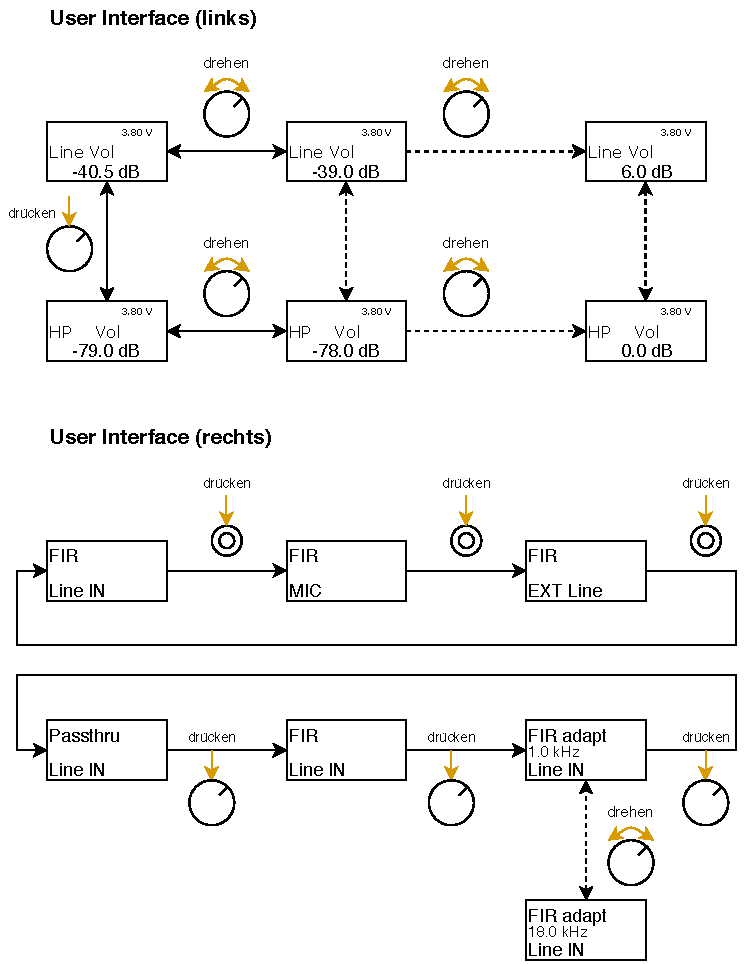
\includegraphics[width=0.75\linewidth]{P5-User-Interface}
	\caption{Das Diagramm zeigt die beiden OLED-Displays mit dem Menu und den Interaktionen}
	\label{pic:P5-User-Interface}
\end{figure}

Mit der linken Seite wird die Lautstärke für Line-Out und Headphone eingestellt.
Auf der rechten Seite, kann einerseits mit dem Button die Input-Quelle selektiert werden und andererseits mit dem Encoder die DSP-Funktion ausgewählt werden. 
Beim Menupunkt \glqq\textit{FIR adapt}\grqq \ kann zusätzlich die Grenzfrequenz des FIR Tiefpassfilters verändert werden.



